%% LyX 1.5.1 created this file.  For more info, see http://www.lyx.org/.
%% Do not edit unless you really know what you are doing.
\documentclass[oneside,english,onecolumn]{book}
\usepackage[T1]{fontenc}
\usepackage[latin1]{inputenc}
\usepackage{geometry}
\geometry{letterpaper,tmargin=1in,bmargin=1in,lmargin=1in,rmargin=1in}
\setcounter{secnumdepth}{3}
\setcounter{tocdepth}{3}
\usepackage{float}
\usepackage{textcomp}
\usepackage{amsmath}

% figures
\usepackage[pdftex]{graphicx}

% we are running pdflatex, so convert .eps files to .pdf
\usepackage{epstopdf}

\usepackage{amssymb}
\IfFileExists{url.sty}{\usepackage{url}}
                      {\newcommand{\url}{\texttt}}
\usepackage[authoryear]{natbib}

\makeatletter

%%%%%%%%%%%%%%%%%%%%%%%%%%%%%% LyX specific LaTeX commands.
\newcommand{\noun}[1]{\textsc{#1}}
%% A simple dot to overcome graphicx limitations
\newcommand{\lyxdot}{.}


%%%%%%%%%%%%%%%%%%%%%%%%%%%%%% Textclass specific LaTeX commands.
\newenvironment{lyxcode}
{\begin{list}{}{
\setlength{\rightmargin}{\leftmargin}
\setlength{\listparindent}{0pt}% needed for AMS classes
\raggedright
\setlength{\itemsep}{0pt}
\setlength{\parsep}{0pt}
\normalfont\ttfamily}%
 \item[]}
{\end{list}}

%%%%%%%%%%%%%%%%%%%%%%%%%%%%%% User specified LaTeX commands.
%\renewcommand{\baselinestretch}{1.5}

% figures
\usepackage[dvips]{epsfig}

\usepackage{wrapfig}


% fonts
\usepackage{times}

% hyperlinks to sections and references
\usepackage[pdftex,bookmarks=true,bookmarksnumbered=true,pdfpagemode=None,pdfstartview=FitH,pdfpagelayout=SinglePage,pdfborder={0 0 0}]{hyperref}

\newcommand{\urlwithparentheses}[1]{(\url{#1})}

% biblio GJI
\bibliographystyle{abbrvnat}

\newcommand{\toall}[1]{\textbf{*** All: #1 ***}}
\newcommand{\tojeroen}[1]{\textbf{*** Jeroen: #1 ***}}
\newcommand{\tobrian}[1]{\textbf{*** Brian: #1 ***}}
\newcommand{\tovala}[1]{\textbf{*** Vala: #1 ***}}
\newcommand{\tovalabrian}[1]{\textbf{*** Vala \& Brian: #1 ***}}
\newcommand{\tovalaqinya}[1]{\textbf{*** Vala \& Qinya: #1 ***}}
\newcommand{\toqinya}[1]{\textbf{*** Qinya: #1 ***}}
\newcommand{\tomin}[1]{\textbf{*** Min: #1 ***}}
\newcommand{\toalessia}[1]{\textbf{*** Alessia: #1 ***}}
\newcommand{\todimitri}[1]{\textbf{*** Dimitri: #1 ***}}

\newcommand{\nexxi}{\mbox{\texttt{NEX\_XI\/}}}
\newcommand{\nexeta}{\mbox{\texttt{NEX\_ETA\/}}}
\newcommand{\nprocxi}{\mbox{\texttt{NPROC\_XI\/}}}
\newcommand{\nproceta}{\mbox{\texttt{NPROC\_ETA\/}}}
\newcommand{\nchunks}{\mbox{\texttt{NCHUNKS\/}}}

% colors to show the corrections
\usepackage[dvipsnames,usenames]{color}

% colors to show the corrections
\newcommand{\red}[1]{\textbf{\textcolor{Red}{#1}}}
\newcommand{\blue}[1]{\textbf{\textcolor{Blue}{#1}}}
\newcommand{\cyan}[1]{\textbf{\textcolor{Cyan}{#1}}}
\newcommand{\green}[1]{\textbf{\textcolor{Green}{#1}}}
\newcommand{\magenta}[1]{\textbf{\textcolor{Magenta}{#1}}}
\newcommand{\orange}[1]{\textbf{\textcolor{Orange}{#1}}}
%\newcommand{\red}[1]{#1}
%\newcommand{\blue}[1]{#1}
%\newcommand{\cyan}[1]{#1}

\usepackage{babel}
\makeatother

\begin{document}
\begin{center}
\thispagestyle{empty}%
\vspace*{-1.8truecm}
\noindent\makebox[\textwidth]{%
\noindent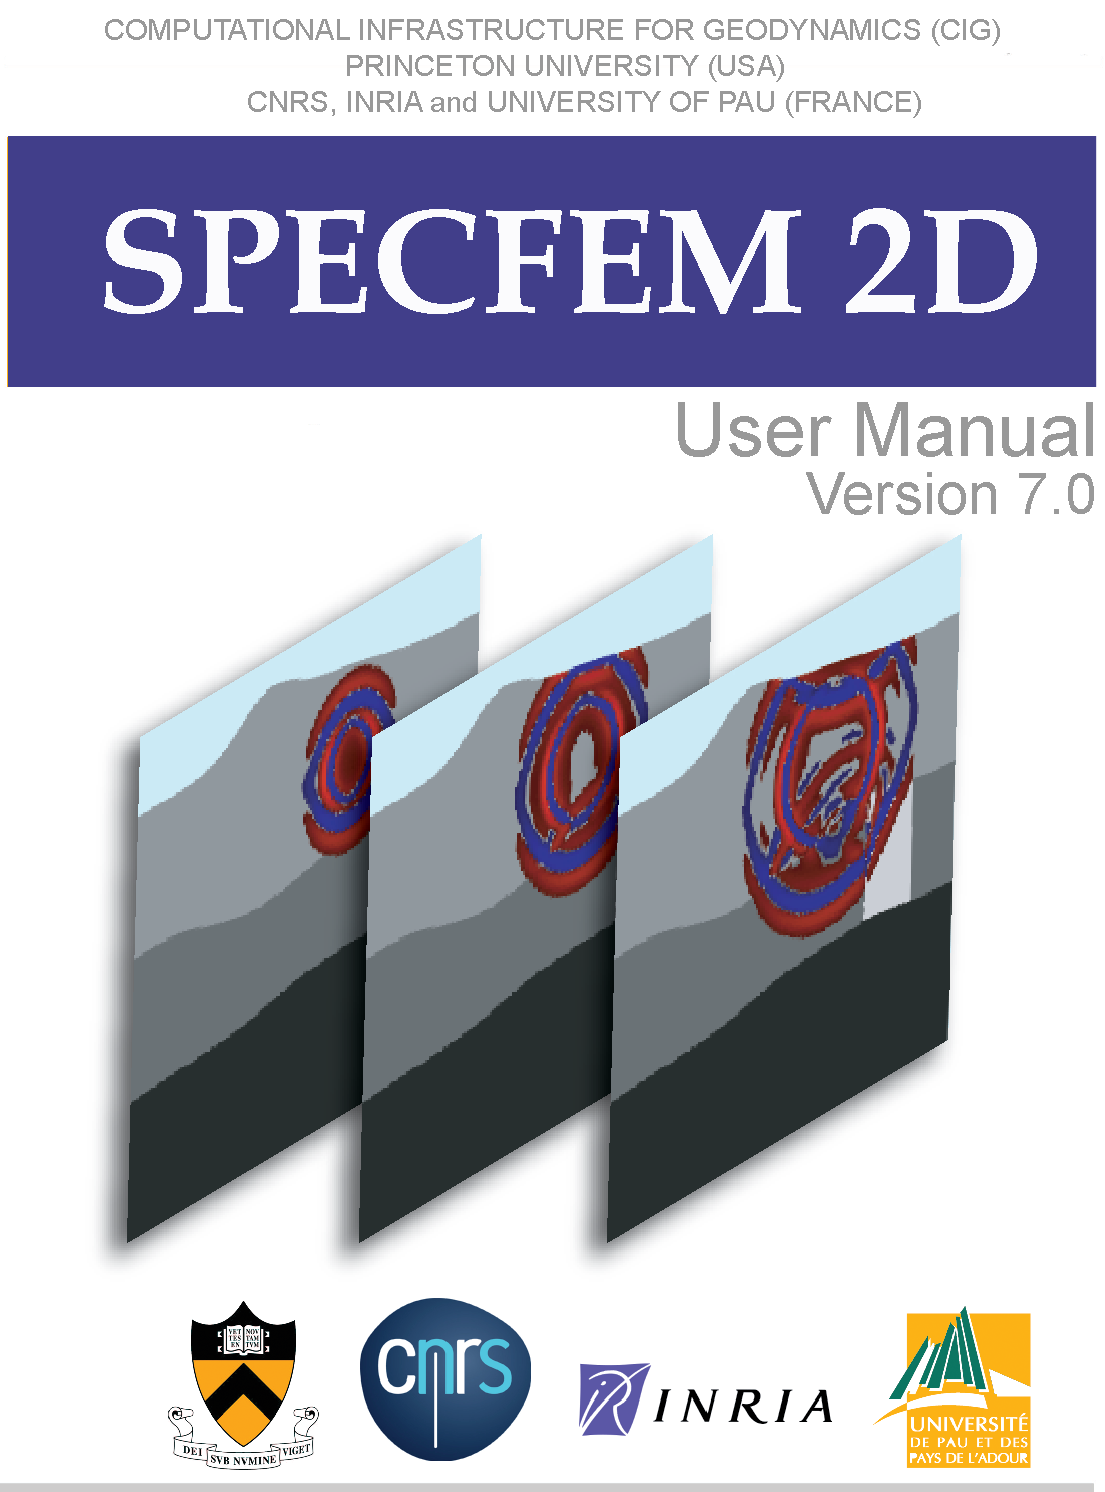
\includegraphics[width=0.83\paperwidth]{figures/specfem_2d-cover.pdf}
}
\end{center}
%
\title{\textbf{SPECFEM2D}\\
\textbf{User Manual}}

\author{$\copyright$ Princeton University (USA) and CNRS and University of Marseille (France)\\
Version 7.0
}

\date{\noindent \today}

\maketitle

\section*{Authors}
The SPECFEM2D package was first developed by Dimitri Komatitsch and Jean-Pierre Vilotte at IPG in Paris (France) from 1995 to 1997
and then by Dimitri Komatitsch at Harvard University (USA), Caltech (USA) and then CNRS and University of Pau (France) from 1998 to 2005.
The story started on March 28, 1995, when Prof. Yvon Maday from CNRS and University of Paris, France, gave a lecture to
Dimitri Komatitsch and Jean-Pierre Vilotte at IPG about the nice properties of the spectral-element method that he had used for
other equations. We are deeply indebted and thankful to him for that.\\

\noindent
Since then it has been developed and maintained by a development team: in alphabetical order,
Paul Cristini,
Dimitri Komatitsch,
Jes\'us Labarta,
Nicolas Le Goff,
Pieyre Le Loher,
Qinya Liu,
Roland Martin,
Ren\'e Matzen,
Christina Morency,
Daniel Peter,
Carl Tape,
Jeroen Tromp,
Jean-Pierre Vilotte,
Zhinan Xie.

\section*{Current and past main participants or main sponsors}

\begin{figure}[htbp]
\noindent \begin{centering}

\includegraphics[width=0.125\textwidth]{figures/logo_cnrs}\vspace*{2truemm}

\includegraphics[width=0.125\textwidth]{figures/logo_princeton}\vspace*{2truemm}

\includegraphics[width=0.15\textwidth]{figures/logo_aix_marseille_universite}\vspace*{0.02truemm}

\includegraphics[width=0.12\textwidth]{figures/logo_CSC_China}\vspace*{0.02truemm}
%%
\includegraphics[width=0.15\textwidth]{figures/logo_ETH}\vspace*{2truemm}  %% did not work on the 2D version

\includegraphics[width=0.15\textwidth]{figures/logo_inria}\vspace*{2truemm}

\includegraphics[width=0.14\textwidth]{figures/logo_UPPA}
\par\end{centering}

\noindent \begin{centering}
%%
\includegraphics[width=0.15\textwidth]{figures/logo_NVIDIA}\vspace*{2truemm}  %% did not work on the 2D version

\includegraphics[width=0.125\textwidth]{figures/logo_IUF}\vspace*{2truemm}

\includegraphics[width=0.135\textwidth]{figures/logo_Caltech}\vspace*{2truemm}

\includegraphics[width=0.135\textwidth]{figures/logo_Harvard}\vspace*{2truemm}

\includegraphics[width=0.135\textwidth]{figures/logo_IPGP}\vspace*{2truemm}
\par\end{centering}

\noindent \begin{centering}

\includegraphics[width=0.119\textwidth]{figures/logo_INGV}\vspace*{2truemm}

\includegraphics[width=0.119\textwidth]{figures/logo_University_of_Toronto}\vspace*{2truemm}

\includegraphics[width=0.112\textwidth]{figures/logo_Univ_Toulouse}\vspace*{2truemm}

\includegraphics[width=0.112\textwidth]{figures/logo_TOTAL}\vspace*{2truemm}

\includegraphics[width=0.130\textwidth]{figures/logo_Fairbanks}
\par\end{centering}
\end{figure}

\newpage{}

\tableofcontents{}

%------------------------------------------------------------------------------------------------%

\chapter{Introduction}

%------------------------------------------------------------------------------------------------%

SPECFEM2D facilitates 2D simulations of
acoustic, (an)elastic, and poroelastic seismic wave propagation.
The 2D spectral-element solver accommodates
regular and unstructured meshes, generated for example by Cubit
\urlwithparentheses{http://cubit.sandia.gov},
Gmsh \urlwithparentheses{http://geuz.org/gmsh}
or GiD \urlwithparentheses{http://www.gid.cimne.upc.es}.
Even mesh creation packages that generate triangles, for instance Delaunay-Voronoi triangulation codes, can be used because each triangle can then easily be decomposed into three quadrangles by linking the barycenter to the center of each edge; while this approach does not generate quadrangles of optimal quality, it can ease mesh creation in some situations and it has been shown that the spectral-element method can very accurately handle distorted mesh elements.\\

With version 7.0, the 2D spectral-element solver accommodates Convolution PML absorbing layers and well as higher-order time schemes
(4th order Runge-Kutta and LDDRK4-6).
Convolution or Auxiliary Differential Equation Perfectly Matched absorbing Layers (C-PML or ADE-PML)
are described in \cite{MaKoEz08,MaKoGe08,MaKo09,MaKoGeBr10,KoMa07}.\\

The solver has adjoint capabilities and can
calculate finite-frequency sensitivity kernels \citep{TrKoLi08,PeKoLuMaLeCaLeMaLiBlNiBaTr11} for acoustic,
(an)elastic, and poroelastic media. The package also considers 2D SH
and P-SV wave propagation. Finally, the solver can run
both in serial and in parallel. See SPECFEM2D
\urlwithparentheses{http://www.geodynamics.org/cig/software/packages/seismo/specfem2d}
for the source code.\\

The SEM is a continuous Galerkin technique \citep{TrKoLi08,PeKoLuMaLeCaLeMaLiBlNiBaTr11}, which can easily be made discontinous \citep{BeMaPa94,Ch00,KoWoHu02,ChCaVi03,LaWaBe05,Kop06,WiStBuGh10,AcKo11}; it is then close to a particular case of the discontinuous Galerkin technique \citep{ReHi73,LeRa74,Arn82,JoPi86,BoMaHe91,FaRi99,HuHuRa99,CoKaSh00,GiHeWa02,RiWh03,MoRi05,GrScSc06,AiMoMu06,BeLaPi06,DuKa06,DeSeWh08,PuAmKa09,WiStBuGh10,DeSe10,EtChViGl10}, with optimized efficiency because of its tensorized basis functions \citep{WiStBuGh10,AcKo11}.
In particular, it can accurately handle very distorted mesh elements \citep{OlSe11}.\\

It has very good accuracy and convergence properties \citep{MaPa89,SePr94,DeFiMu02,Coh02,DeSe07,SeOl08,MeStTh12}.
The spectral element approach admits spectral rates of convergence and allows exploiting $hp$-convergence schemes.
It is also very well suited to parallel implementation on very large supercomputers \citep{KoTsChTr03,TsKoChTr03,KoLaMi08a,CaKoLaTiMiLeSnTr08,KoViCh10}
as well as on clusters of GPU accelerating graphics cards \citep{KoMiEr09,KoErGoMi10,Kom11}.
Tensor products inside each element can be optimized to reach very high efficiency \citep{DeFiMu02}, and mesh point and element numbering can be optimized to reduce processor cache misses and improve cache reuse \citep{KoLaMi08a}. The SEM can also handle triangular (in 2D) or tetrahedral (in 3D) elements \citep{WinBoyd96,TaWi00,KoMaTrTaWi01,Coh02,MeViSa06} as well as mixed meshes, although with increased cost and reduced accuracy in these elements, as in the discontinuous Galerkin method.\\

Note that in many geological models in the context of seismic wave propagation studies
(except for instance for fault dynamic rupture studies, in which very high frequencies or supershear rupture need to be modeled near the fault, see e.g. \cite{BeGlCrViPi07,BeGlCrVi09,PuAmKa09,TaCrEtViBeSa10})
a continuous formulation is sufficient because material property contrasts are not drastic and thus
conforming mesh doubling bricks can efficiently handle mesh size variations \citep{KoTr02a,KoLiTrSuStSh04,LeChLiKoHuTr08,LeChKoHuTr09,LeKoHuTr09}.\\

For a detailed introduction to the SEM as applied to regional
seismic wave propagation, please consult \citet{PeKoLuMaLeCaLeMaLiBlNiBaTr11,TrKoLi08,KoVi98,KoTr99,ChKoViCaVaFe07} and
in particular \citet{LeKoHuTr09,LeChKoHuTr09,LeChLiKoHuTr08,GoAmTaCaSmSaMaKo09,WiKoScTr04,KoLiTrSuStSh04}.
A detailed theoretical analysis of the dispersion
and stability properties of the SEM is available in \citet{Coh02}, \citet{DeSe07}, \citet{SeOl07}, \citet{SeOl08} and \citet{MeStTh12}.\\

The SEM was originally developed in computational fluid dynamics \citep{Pat84,MaPa89}
and has been successfully adapted to address problems in seismic wave propagation.
Early seismic wave propagation applications of the SEM, utilizing Legendre basis functions and a
perfectly diagonal mass matrix, include \cite{CoJoTo93}, \cite{Kom97},
\cite{FaMaPaQu97}, \cite{CaGa97}, \cite{KoVi98} and \cite{KoTr99},
whereas applications involving Chebyshev basis functions and a nondiagonal mass matrix
include \cite{SePr94}, \cite{PrCaSe94} and \cite{SePrPr95}.\\

All SPECFEM2D software is written in Fortran2003 with full portability
in mind, and conforms strictly to the Fortran2003 standard. It uses
no obsolete or obsolescent features of Fortran. The package uses
parallel programming based upon the Message Passing Interface (MPI)
\citep{GrLuSk94,Pac97}.\\

The next release of the code will include support for GPU graphics card acceleration \citep{KoMiEr09,KoErGoMi10,MiKo10,Kom11}.\\

%------------------------------------------------------------------------------------------------%
\section{Citation}
%------------------------------------------------------------------------------------------------%

If you use this code for your own research, please cite at least one article
written by the developers of the package, for instance:
\newline
\cite{TrKoLi08,PeKoLuMaLeCaLeMaLiBlNiBaTr11}
or
\cite{VaCaSaKoVi99, LeChKoHuTr09, LeChLiKoHuTr08, LeKoHuTr09, KoErGoMi10, KoMiEr09,
LiPoKoTr04, ChKoViCaVaFe07, KoVi98, KoTr99, KoLiTrSuStSh04, MoTr08}
and/or other articles from \url{http://komatitsch.free.fr/publications.html}
\newline

If you use the kernel capabilities of the code, please cite at least one article
written by the developers of the package, for instance:
\newline
\cite{TrKoLi08,PeKoLuMaLeCaLeMaLiBlNiBaTr11,LiTr06, MoLuTr09}
\newline

If you use the SCOTCH / CUBIT non-structured capabilities, please also cite:
\newline
\cite{MaKoBlLe08}
\newline

The corresponding Bib\TeX{} entries may be found
in file \texttt{doc/USER\_MANUAL/bibliography.bib}.



%------------------------------------------------------------------------------------------------%
\section{Support}
%------------------------------------------------------------------------------------------------%

This material is based upon work supported by the USA National Science
Foundation under Grants No. EAR-0406751 and EAR-0711177, by the French
CNRS, French INRIA Sud-Ouest MAGIQUE-3D, French ANR NUMASIS under
Grant No. ANR-05-CIGC-002, and European FP6 Marie Curie International
Reintegration Grant No. MIRG-CT-2005-017461.
Any opinions, findings, and conclusions or recommendations expressed in this material are
those of the authors and do not necessarily reflect the views of the
USA National Science Foundation, CNRS, INRIA, ANR or the European
Marie Curie program.



%------------------------------------------------------------------------------------------------%

\chapter{\label{cha:Getting-Started}Getting Started}

%------------------------------------------------------------------------------------------------%

The SPECFEM2D software package comes in a gzipped tar ball. In the
directory in which you want to install the package, type
\begin{lyxcode}
{\small tar~-zxvf~SPECFEM2D\_7.0.0.tar.gz}{\small \par}
\end{lyxcode}
The directory \texttt{SPECFEM2D-7.0.0/} will then contain
the source code. In the following, we will refer to this directory as the root directory \texttt{SPECFEM2D/}. \\

We recommend that you add {\texttt{ulimit -S -s unlimited}} to your {\texttt{.bash\_profile}} file and/or {\texttt{limit stacksize unlimited }} to your {\texttt{.cshrc}} file to suppress any potential limit to the size of the Unix stack.\\

Then, to configure the software for your system, run the
\texttt{configure} shell script. This script will attempt to guess
the appropriate configuration values for your system. However, at
a minimum, it is recommended that you explicitly specify the appropriate
command names for your Fortran compiler (another option is to define FC, CC and MPIF90 in your .bash\_profile
or your .cshrc file):
\begin{lyxcode}
./configure~FC=ifort~
\end{lyxcode}

If you want to run in parallel, i.e., using more than one processor core, then you would type
\begin{lyxcode}
./configure~FC=ifort~MPIFC=mpif90~-{}-with-mpi
\end{lyxcode}

Before running the \texttt{configure} script, you should probably edit file \texttt{flags.guess} to make sure that it contains the best compiler options for your system. Known issues or things to check are:

\begin{description}
\item [{\texttt{Intel ifort compiler}}] See if you need to add \texttt{-assume byterecl} for your machine.
\item [{\texttt{IBM compiler}}] See if you need to add \texttt{-qsave} or \texttt{-qnosave} for your machine.
\item [{\texttt{Mac OS}}] You will probably need to install \texttt{XCODE}.
In addition, the \texttt{clock\_gettime} routine, which is used by the \texttt{SCOTCH} library that we use, does not exist in Mac OS.
You will need to replace it with \texttt{clock\_get\_time} if you want to use \texttt{SCOTCH}.
\item [{\texttt{IBM Blue Gene machines}}] Please refer to the manual of SPECFEM3D\_Cartesian, which contains detailed instructions on how to run on Blue Gene.
\end{description}

The SPECFEM2D software package relies on the SCOTCH library to partition meshes.
The SCOTCH library \citep{PeRo96}
provides efficent static mapping, graph and mesh partitioning routines. SCOTCH is a free software package developed by
Fran\c {c}ois Pellegrini et al. from LaBRI and INRIA in Bordeaux, France, downloadable from the web page \url{https://gforge.inria.fr/projects/scotch/}.
In case no SCOTCH libraries can be found on the system, the configuration will bundle the version provided with the source code for compilation.
The path to an existing SCOTCH installation can to be set explicitly with the option \texttt{-{}-with-scotch-dir}.
Just as an example:
\begin{lyxcode}
./configure~FC=ifort~MPIFC=mpif90~-{}-with-mpi~-{}-with-scotch-dir=/opt/scotch
\end{lyxcode}

If you use the Intel ifort compiler to compile the code, we recommend that you use the Intel icc C compiler to compile Scotch, i.e., use:
\begin{lyxcode}
./configure~CC=icc~FC=ifort~MPIFC=mpif90
\end{lyxcode}

For further details about the installation of SCOTCH,
go to subdirectory \texttt{scotch\_5.1.11/} and read \texttt{INSTALL.txt}. You may want to download more recent versions of SCOTCH in the future from \urlwithparentheses{http://www.labri.fr/perso/pelegrin/scotch/scotch_en.html} . Support for the METIS graph partitioner has been discontinued because SCOTCH is more recent and performs better.

Edit the \texttt{Makefile} for more specific modifications. Especially, there are several options available :\\
\texttt{-DUSE\_MPI} compiles with use of an MPI library. \\
\texttt{-DUSE\_SCOTCH} enables use of graph partitioner SCOTCH.

After these steps, go back to the main directory of SPECFEM2D/ and type
\begin{lyxcode}
make
\end{lyxcode}
to create all executables which will be placed into the folder \texttt{./bin/}.

If you run very large meshes on a relatively small number
of processors, the memory size needed on each processor might become
greater than 2 gigabytes, which is the upper limit for 32-bit addressing.
In this case, on some compilers you may need to add \texttt{``-mcmodel=medium}'' or \texttt{``-mcmodel=medium -shared-intel}''
to the configure options of CFLAGS, FCFLAGS and LDFLAGS otherwise the compiler will display an error
message (for instance \texttt{``relocation truncated to fit: R\_X86\_64\_PC32 against .bss''} or something similar);
on an IBM machine with the \texttt{xlf} and \texttt{xlc} compilers, using \texttt{-q64} is usually sufficient.

By default, the solver runs in single precision. This is fine for most application, but if for some reason
you want to run the solver in double precision, run the \texttt{configure} script with option \texttt{``--enable-double-precision}''.
Keep in mind that this will of course double total memory size and will also make the solver around 20 to 30\% slower
on many processors.

If your compiler has problems with the \texttt{use mpi} statements that are used in the code, use the script called 
\texttt{replace\_use\_mpi\_with\_include\_mpif\_dot\_h.pl} in the root directory to replace all of them with \texttt{include 'mpif.h'} automatically.

\section{Visualizing the subroutine calling tree of the source code}

Packages such as \texttt{doxywizard} can be used to visualize the subroutine calling tree of the source code.
\texttt{Doxywizard} is a GUI front-end for configuring and running \texttt{doxygen}.

%------------------------------------------------------------------------------------------------%

\chapter{Mesh Generation}

%------------------------------------------------------------------------------------------------%

%------------------------------------------------------------------------------------------------%
\section{How to use SPECFEM2D}
%------------------------------------------------------------------------------------------------%

\begin{figure}[htbp]
\noindent \begin{centering}
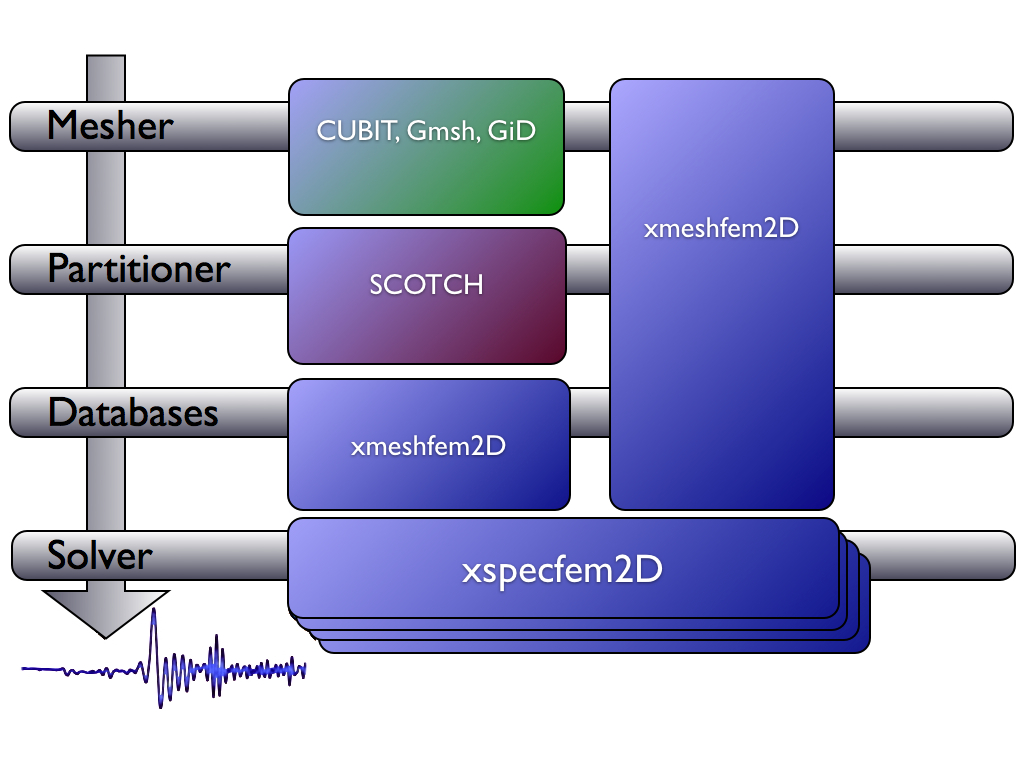
\includegraphics[width=.6\textwidth]{figures/workflow.jpg}
\par\end{centering}

\caption{Schematic workflow for a SPECFEM2D simulation. The executable \texttt{xmeshfem2D} creates the GLL mesh points and assigns specific model parameters. The executable \texttt{xspecfem2D} solves the seismic wave propagation.}

\label{fig:workflow.databases}
\end{figure}


\noindent
To run the mesher, please follow these steps:

\begin{itemize}

\item edit the input file \texttt{DATA/Par\_file}, which describes the simulation.
The default \texttt{DATA/Par\_file} provided with the code contains detailed comments and should be almost self-explanatory
(note that older \texttt{DATA/Par\_file} files provided in the \texttt{EXAMPLES} directory work fine but some of the comments
they contain may be obsolete or even wrong; thus refer to the default \texttt{DATA/Par\_file} instead for reliable explanations).
If you need more details we do not have a detailed description of all the parameters for the 2D version in this manual
but you can find useful information in the manuals of the 3D versions, since many parameters and the general philosophy is similar. They are available at
\urlwithparentheses{http://geodynamics.org/wsvn/cig/seismo/3D} in subdirectories \texttt{USER\_MANUAL/}.
To create acoustic (fluid) regions, just set the S wave speed to zero and the code will see that these elements are fluid and switch to the right equations there automatically, and automatically match them with the solid regions

\item if you are using an external mesher (like GID or CUBIT / Trelis), you should set \texttt{read\_external\_mesh} to \texttt{.true.}:
	\begin{description}
     \item[\texttt{mesh\_file}] is the file describing the mesh : first line is the number of elements, then a list of 4 nodes (quadrilaterals only) forming each elements on each line.

     \item[\texttt{nodes\_coords\_file}] is the file containing the coordinates ($x$ and $z$) of each node: number of nodes on the first line, then coordinates x and z on each line.

     \item[\texttt{materials\_file}] is the number of the material for every elements : an integer ranging from 1 to nbmodels on each line.

     \item[\texttt{free\_surface\_file}] is the file describing the edges forming the acoustic free surface: number of edges on the first line, then on each line: number of the element, number of nodes forming the free surface (1 for a point, 2 for an edge), the nodes forming the free surface for this element. If you do not want any free surface, just put 0 on the first line.

     \item[\texttt{absorbing\_surface\_file}] is the file describing the edges forming the absorbing boundaries:
number of edges on the first line, then on each line: number of the element, number of nodes forming the absorbing edge (must always be equal to 2),
the two nodes forming the absorbing edge for this element, and then the type of absorbing edge: 1 for BOTTOM, 2 for RIGHT, 3 for TOP and 4 for LEFT.
Only two nodes per element can be listed, i.e., the second parameter of each line must always be equal to 2.
If one of your elements has more than one edge along a given absorbing contour
(e.g., if that contour has a corner) then list it twice,
putting the first edge on the first line and the second edge on the second line.
Do not list the same element with the same absorbing edge twice or more, otherwise absorption will not be correct because the edge integral
will be improperly subtracted several times.
If one of your elements has a single point along the absording contour rather than a full edge, do NOT list it
(it would have no weight in the contour integral anyway because it would consist of a single point).
If you use 9-node elements, list only the first and last points of the edge and not the intermediate point
located around the middle of the edge; the right 9-node curvature will be restored automatically by the code.

     \item[\texttt{tangential\_detection\_curve\_file}] contains points describing the envelope, used for \texttt{source\_normal\_to\_surface} and \texttt{rec\_normal\_to\_surface}. Should be fine grained, and ordained clockwise. Number of points on the first line, then (x,z) coordinates on each line.
	\end{description}

\item if you have compiled with MPI, you must specify the number of processes.

\end{itemize}
Then type
\begin{lyxcode}
./bin/xmeshfem2D
\end{lyxcode}
to create the mesh (which will be stored in directory \texttt{OUTPUT\_FILES/}). \texttt{xmeshfem2D} is serial; it will output several files called \texttt{Database??????}, one for each process.

%%
\begin{figure}[htbp]
\noindent \begin{centering}
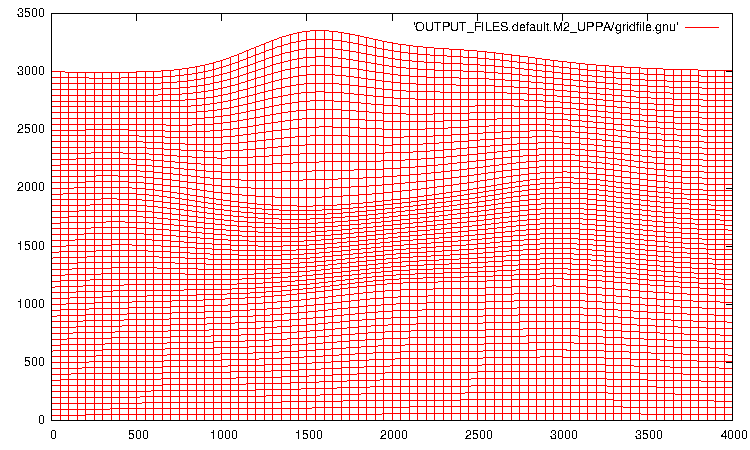
\includegraphics[width=3in]{figures/example-gridfile.pdf}
\par\end{centering}
\caption{Example of a grid file generated by \texttt{xmeshfem2D} and visualized with gnuplot
(within gnuplot, type `\texttt{plot "OUTPUT\_FILES/gridfile.gnu" w l}`).}
\label{fig:example.mesh}
\end{figure}
%%

Regarding mesh point numbering in the files created by the mesher, we use the classical convention of 4-node and 9-node finite elements:
\begin{verbatim}
         4 . . . . 7 . . . . 3
         .                   .
         .         eta       .
         .         |         .
         8         9--xi     6
         .                   .
         .                   .
         .                   .
         1 . . . . 5 . . . . 2
\end{verbatim}
\noindent
the local coordinate system being $\xi$ and $\eta$ (\texttt{xi} and \texttt{eta}).
Note that this convention is used to describe the geometry only. In the solver the wave field is then described based on high-order Lagrange interpolants
at Gauss-Lobatto-Legendre points, as is classical in spectral-element methods.

\section{How to use Gmsh to generate an external mesh}

Gmsh%
\footnote{freely available at the following address : http://www.geuz.org/gmsh/%
} is a 3D finite element grid generator which can be used for the generation
of quadrangle and hexahedral meshes. It is therefore a good candidate
for generating meshes which can be processed by SPECFEM2D. Only two
modules of Gmsh are of interest for the SPECFEM2D users : the geometry
and the mesh modules. An example is given in directory \texttt{EXAMPLES/Gmsh\_example}
which illustrates the generation of an external mesh using these two
modules. The model, which is considered, consists of a homogeneous
square containing two circles filled with a different material.

The geometry is generated by loading file \texttt{SqrCirc.geo} into
Gmsh. The end of the \texttt{.geo} file contains several lines which
are required in order to define the sides of the box and the media.
This is done using the following conventions :

\medskip{}


\texttt{\textit{Physical Line(\textquotedbl{}Top\textquotedbl{}) =
\{1\}; }}{\textsf{\textit{\small line corresponding
to the top of the box}}}{\small \par}

\texttt{\textit{Physical Line(\textquotedbl{}Left\textquotedbl{})
= \{2\}; }}{\textsf{\textit{\small line
corresponding to the left side of the box}}}{\small \par}

\texttt{\textit{Physical Line(\textquotedbl{}Bottom\textquotedbl{})
= \{3\}; }}{\textsf{\textit{\small line
corresponding to the bottom of the box}}}{\small \par}

\texttt{\textit{Physical Line(\textquotedbl{}Right\textquotedbl{})
= \{4\}; }}{\textsf{\textit{\small line
corresponding to the right side of the box}}}{\small \par}

\texttt{\textit{Physical Surface(\textquotedbl{}M1\textquotedbl{})
= \{10\}; }}{\textsf{\textit{\small surrounding
medium}}}{\small \par}

\texttt{\textit{Physical Surface(\textquotedbl{}M2\textquotedbl{})
= \{11,12\}; }}{\textsf{\textit{\small interior
of the two circles}}}{\small \par}

\medskip{}


For instance, if you want to fill the two circles with two different
materials, you will have to write :

\medskip{}


\texttt{\textit{Physical Surface(\textquotedbl{}M1\textquotedbl{})
= \{10\}; }}{\textsf{\textit{\small surrounding
medium}}}{\small \par}

\texttt{\textit{Physical Surface(\textquotedbl{}M2\textquotedbl{})
= \{11\};}}{\textsf{\textit{\small{} interior
of the big circle}}}{\small \par}

\texttt{\textit{Physical Surface(\textquotedbl{}M3\textquotedbl{})
= \{12\};}}{\textsf{\textit{\small{} interior
of the small circle}}}{\small \par}

\medskip{}


and, consequently, you will have to define a new medium numbered \texttt{3}
in the \texttt{Par\_file}.

\begin{figure}[htbp]
\centerline{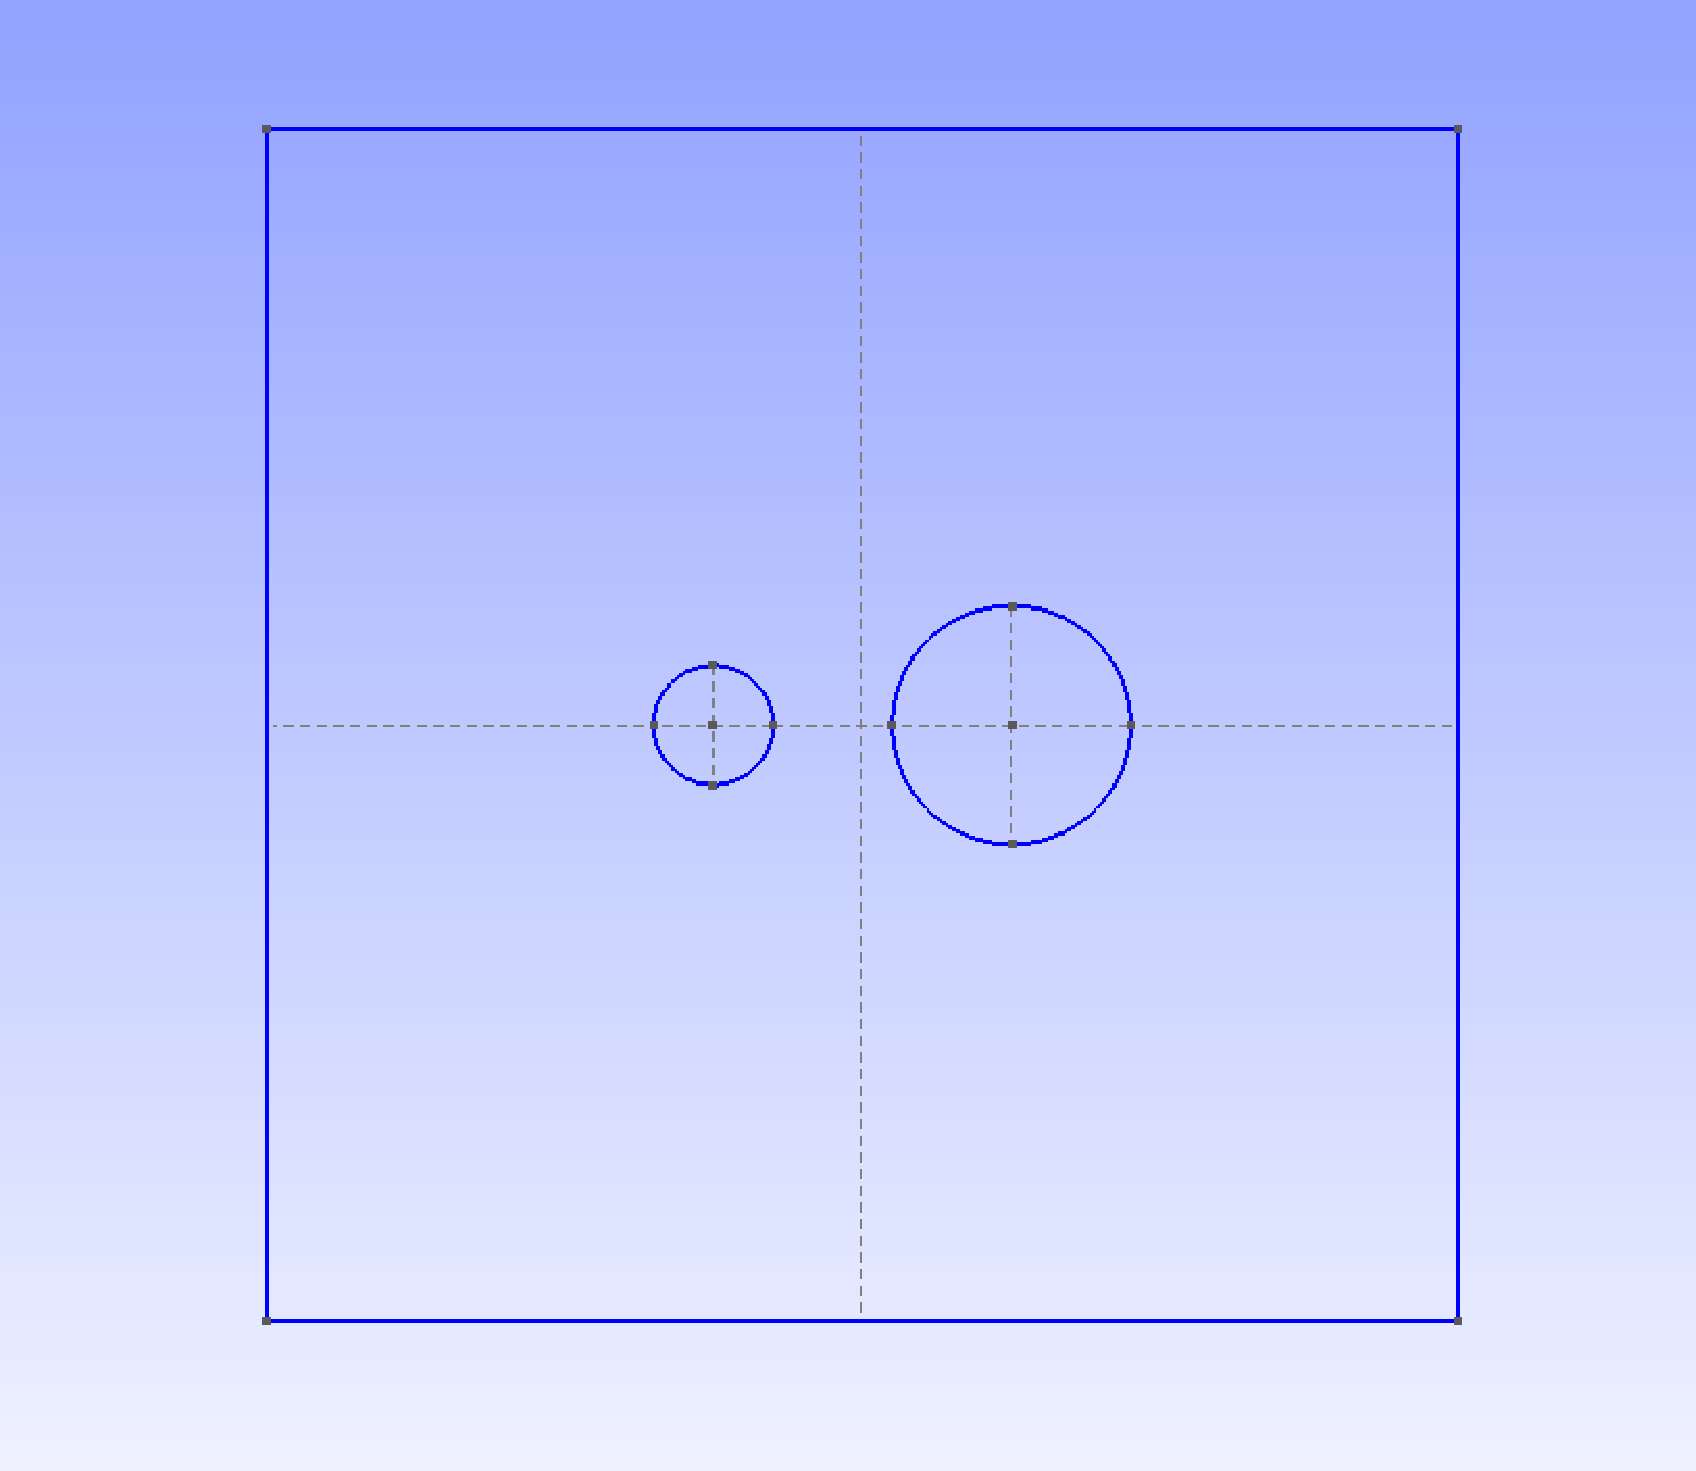
\includegraphics[width=0.481\columnwidth]{figures/Gmsh_geo}\hspace*{2mm}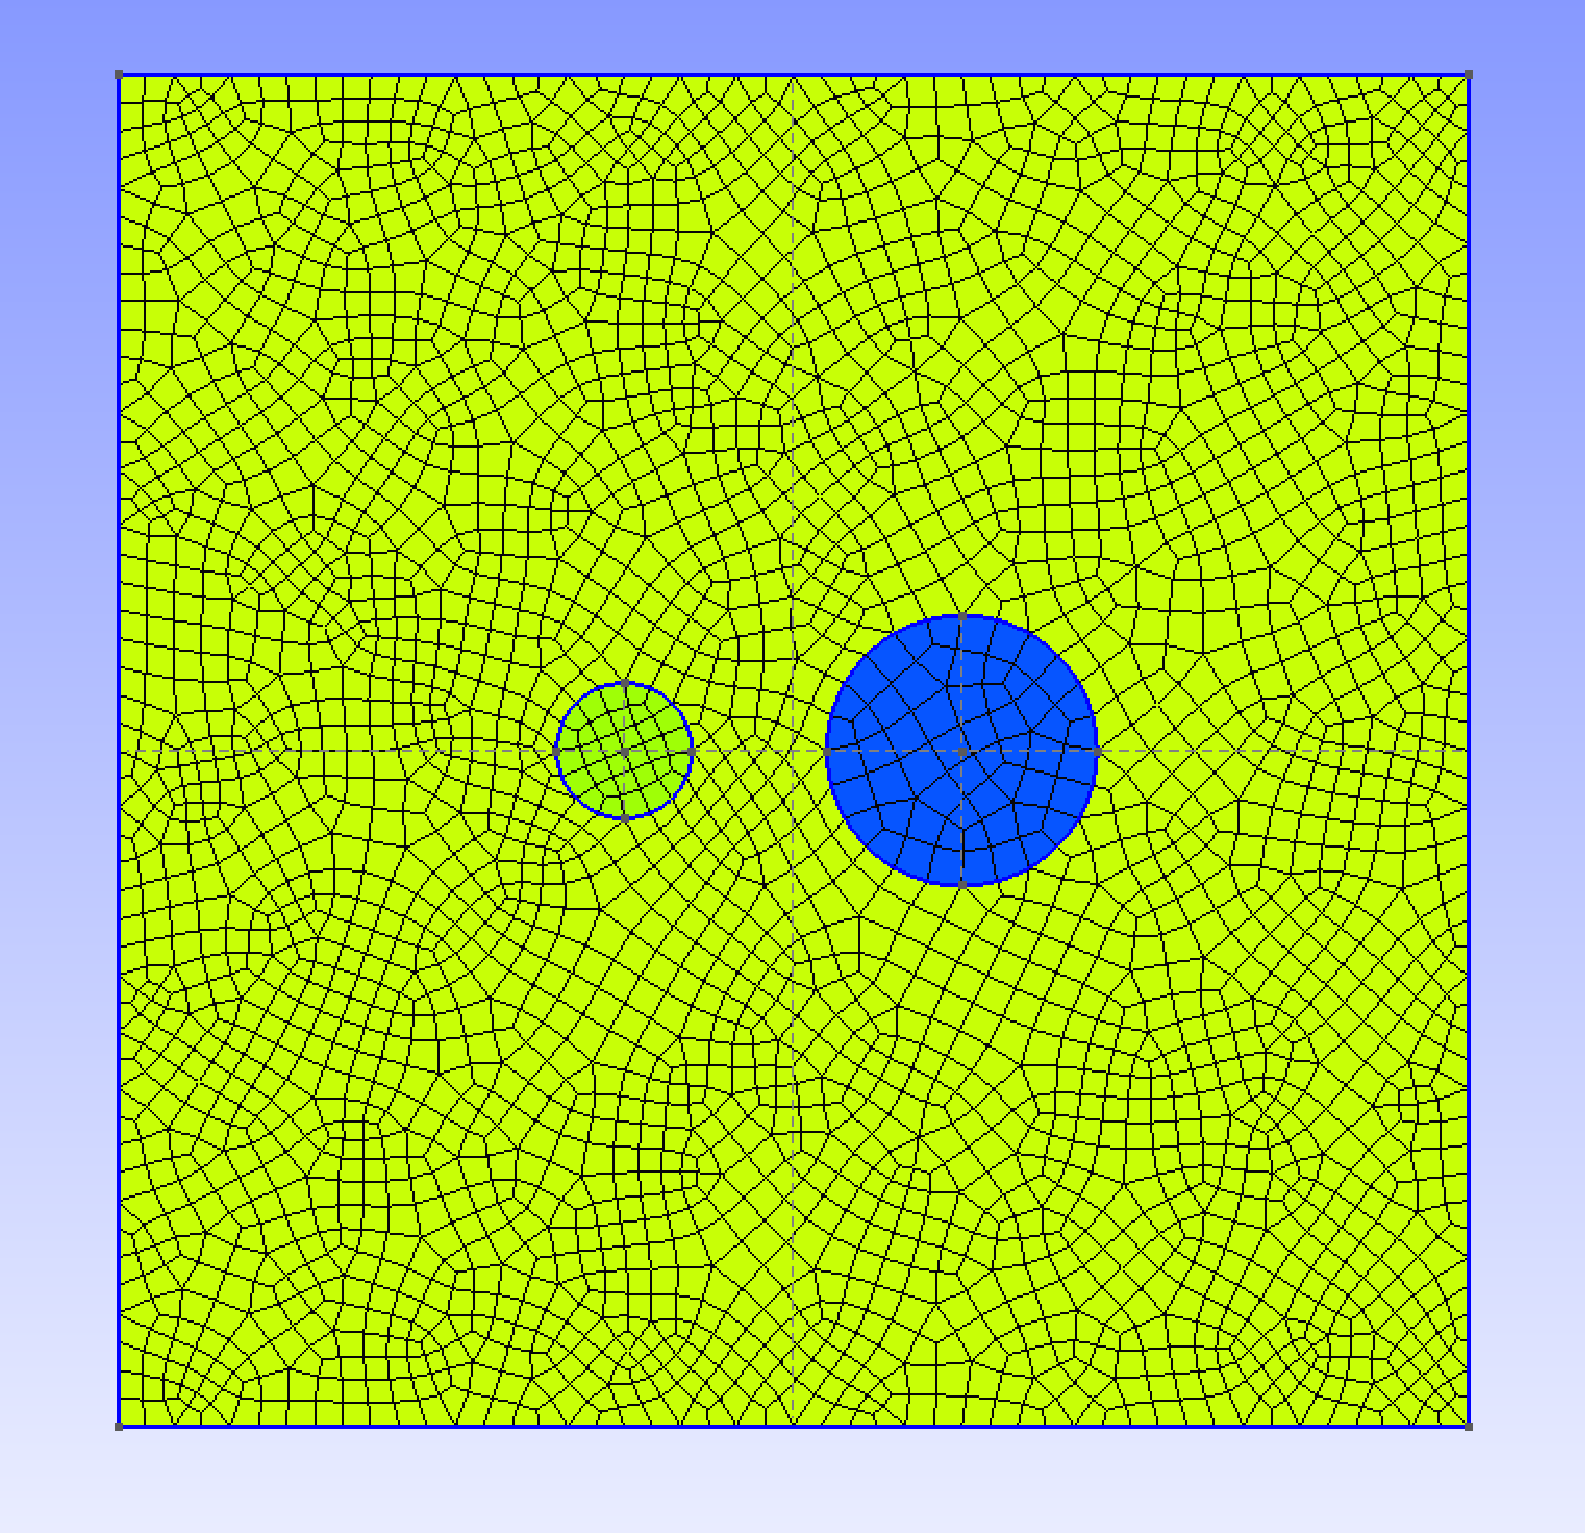
\includegraphics[width=0.43\columnwidth]{figures/Gmsh_Msh}}
\caption{Geometry and mesh of the two circle model generated with Gmsh\label{fig:Gmsh-example}}
\end{figure}


Then, a 2D mesh can be created and saved after selecting the appropriate
options in Gmsh : \texttt{All quads} in \texttt{Subdivision algorithm}
and \texttt{1} or \texttt{2} in \texttt{Element order} whether you
want a 4 or 9 node mesh. This operation will generate a \texttt{SqrCirc.msh}
file which must be processed to get all the files required by SPECFEM2D
when using an external mesh (see previous section). This is done by
running a python script called LibGmsh2Specfem.py, located in directory UTILS/Gmsh:
\begin{lyxcode}
python~LibGmsh2Specfem.py~SqrCirc~-t~A~-b~A~-r~A~-l~A
\end{lyxcode}
Where the options \texttt{-t}, \texttt{-b},\texttt{ -r} and \texttt{-l}
represent the different sides of the model (top, bottom, right and
left) and can take the values \texttt{A} or \texttt{F} if the corresponding
side is respectively absorbing or free. All boundaries are absorbing
by default. The connections of the generated filenames to the filenames
indicated in the previous section are :
\begin{itemize}
\item \texttt{Mesh\_SqrCirc} is the \texttt{\textbf{mesh\_file}}
\item \texttt{Material\_SqrCirc} is the \texttt{\textbf{material\_file}}
\item \texttt{Nodes\_SqrCirc} is the\texttt{ }\texttt{\textbf{nodes\_coords\_file}}
\item \texttt{Surf\_abs\_SqrCirc} is the \texttt{\textbf{absorbing\_surface\_file}}
\item \texttt{Surf\_free\_SqrCirc} is the \texttt{\textbf{free\_surface\_file}}
\end{itemize}
In addition, four files like \texttt{free\_surface\_file} corresponding
to the sides of the model are generated.\\

If you use CPML, an additional file listing the CPML elements is needed.
Its first line is the total number of
CPML elements, and then a list of all the CPML elements, one per line.
The format of these lines is: in the first column the CPML element number, and in the second column a flag as follows:

\begin{table}[hb]
\caption{Definition of flags for CPML elements}
% title of Table
\centering
% used for centering table
\begin{tabular}{c l}
% centered columns (4 columns)
\hline\hline
%inserts double horizontal lines
Flag& Meaning\\ [0.5ex]
% inserts table
%heading
\hline
% inserts single horizontal line
1 & element belongs to a X CPML layer only (either in Xmin or in Xmax)\\
2 & element belongs to a Y CPML layer only (either in Ymin or in Ymax)\\
3 & element belongs to both a X and a Y CPML layer (i.e., to a CPML corner)\\ [1ex]
% [1ex] adds vertical space
\hline
%inserts single line
\end{tabular}
\label{table:CPMLflags}
% is used to refer this table in the text
\end{table}

In order to see how to add PML layers to a mesh / model created with an external mesher such as `Gmsh', see the examples in directory
EXAMPLES/CPML\_absorbing\_layers.

If you use PML, the mesh elements that belong to the PML layers can be acoustic or elastic, but not viscoelastic nor poroelastic.
Then, when defining your model, you should define these absorbing elements as either acoustic or elastic.
In you forget to do that, the code will fix the problem by automatically converting the viscoelastic or poroelastic PML
elements to elastic. This means that strictly speaking the PML layer will not be perfectly matched any more, since the physical
model will change from viscoelastic or poroelastic to elastic at the entrance of the PML, but in practice this is sufficient and
produces only tiny / negligible spurious reflections.

If you use PML and an external velocity and density model (for instance setting flag "READ\_EXTERNAL\_SEP\_FILE" to .true.),
you should be careful because mathematically a PML cannot handle heterogeneities along the
normal to the PML edge inside the PML layer. This comes from the fact that the damping profile
that is defined assumes a constant velocity and density model along the normal
direction.

Thus, you need to modify your velocity and density model in order for it to be 1D inside
the PML, as shown in Figure~\ref{fig:modify_external_velocity_model_to_use_PML}.

This applies to the bottom layer as well; there you should make sure
that your model is 1D and thus constant along the vertical direction.

To summarize, only use a 2D velocity and density model inside the physical region, and in
all the PML layers extend it by continuity from its values along the
inner PML edge.

%%
\begin{figure}[htbp]
\noindent \begin{centering}
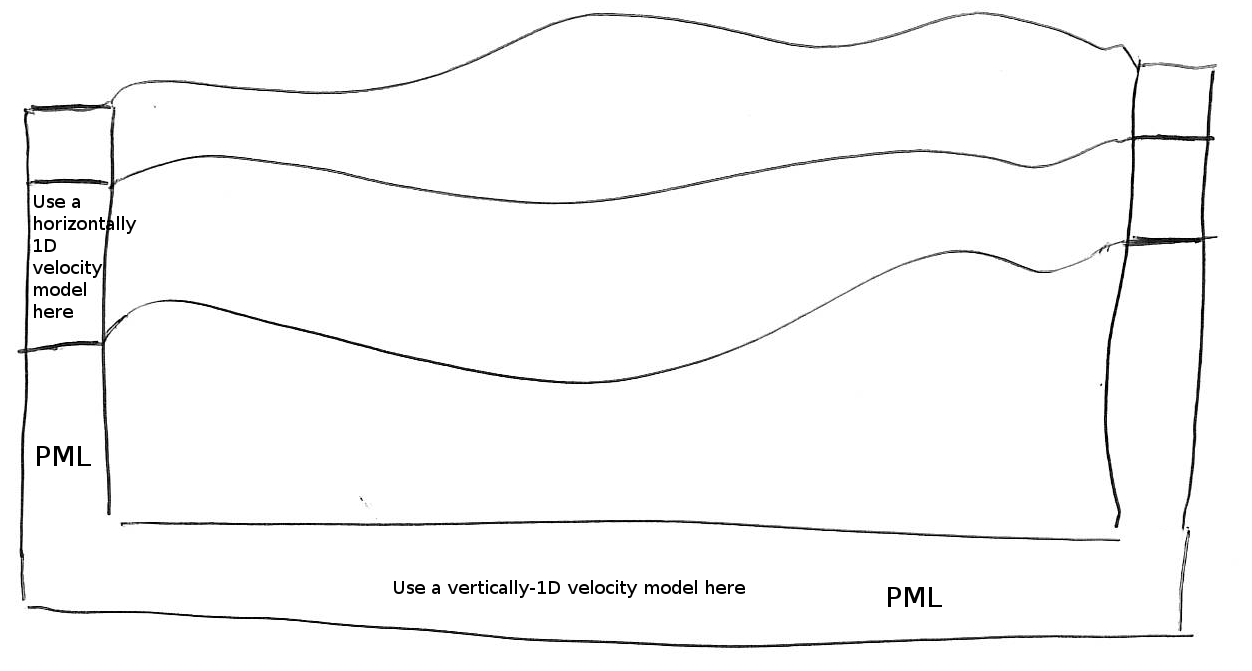
\includegraphics[width=3in]{figures/how_to_use_PML_when_READ_EXTERNAL_SEP_FILE_is_true.png}
\par\end{centering}
\caption{How to modify your external 2D velocity and density model in order to use PML.
Such a modification is not needed when using Stacey absorbing boundary conditions (but such conditions
are significantly less efficient).}
\label{fig:modify_external_velocity_model_to_use_PML}
\end{figure}
%%

%------------------------------------------------------------------------------------------------%
\section{Controlling the quality of an external mesh}
%------------------------------------------------------------------------------------------------%

To examine the quality of the elements in your externally build mesh, type
\begin{lyxcode}
./bin/xcheck\_quality\_external\_mesh
\end{lyxcode}
(and answer "3" to the first question asked).
This code will tell you which element in the whole mesh has the worst quality (maximum skewness, i.e. maximum deformation of the element angles) and it should be enough to modify this element with the external software package used for the meshing, and
to repeat the operation until the maximum skewness of the whole mesh is less or equal to about 0.75 (above is dangerous: from 0.75 to 0.80 could still work, but if there is a single element above 0.80 the mesh should be improved).

The code also shows a histogram of 20 classes of skewness which tells how many element are above the skewness = 0.75, and to which percentage of the total this amounts. To see this histogram, you could type:
\begin{lyxcode}
gnuplot plot\_mesh\_quality\_histogram.gnu
\end{lyxcode}
This tool is useful to estimate the mesh quality and to see it evolve along the successive corrections.

%------------------------------------------------------------------------------------------------%
\section{Controlling how the mesh samples the wave field}
%------------------------------------------------------------------------------------------------%

To examine (using Gnuplot) how the mesh samples the wave field, type
\begin{lyxcode}
gnuplot plot\_points\_per\_wavelength\_histogram.gnu
\end{lyxcode}
%
and also check the following histogram printed on the screen or in the output file:
%
\begin{lyxcode}
 histogram of min number of points per S wavelength
   (P wavelength in acoustic regions)\\
 (too small: poor resolution of calculations -
  too big = wasting memory and CPU time)\\
 (threshold value is around 4.5 points per wavelength
  in elastic media and 5.5 in acoustic media)
\end{lyxcode}

\noindent If you see that you have a significant number of mesh elements below the threshold indicated, then your simulations
will not be accurate and you should create a denser mesh. Conversely, if you have a significant number of mesh elements above the threshold indicated,
the mesh your created is too dense, it will be extremely accurate but the simulations will be slow; using a coarser mesh would be sufficient and would lead to faster simulations.

%------------------------------------------------------------------------------------------------%

\chapter{Running the Solver xspecfem2D}

%------------------------------------------------------------------------------------------------%

To run the solver, type:
\begin{lyxcode}
./bin/xspecfem2D
\end{lyxcode}
to run the main solver (use \texttt{mpirun} or equivalent if you compiled with parallel support). This will output the seismograms and snapshots of the wave fronts at different time steps in directory \texttt{OUTPUT\_FILES/}. To visualize them, type "\texttt{gs OUTPUT\_FILES/vect*.ps}" to see the Postscript files (in which the wave field is represented with small arrows, fluid/solid matching interfaces with a thick pink line, and absorbing edges with a thick green line) and "\texttt{gimp OUTPUT\_FILES/image*.gif}" to see the color snapshot showing a pixelized image of one of the two components of the wave field (or pressure, depending on what you have selected for the output in \texttt{DATA/Par\_file}).


%%
\begin{figure}[htbp]
\noindent \begin{centering}
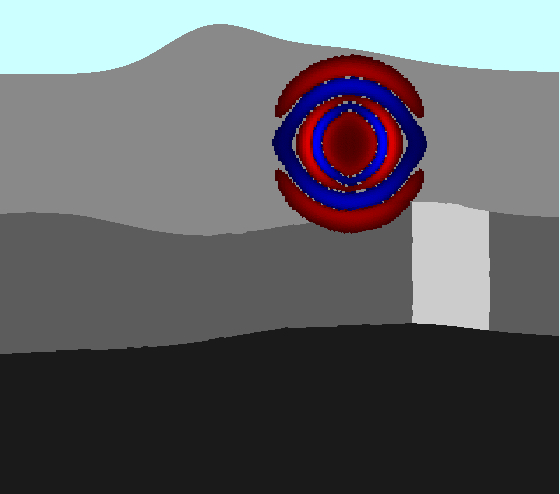
\includegraphics[width=2in]{figures/image0000300.jpg}
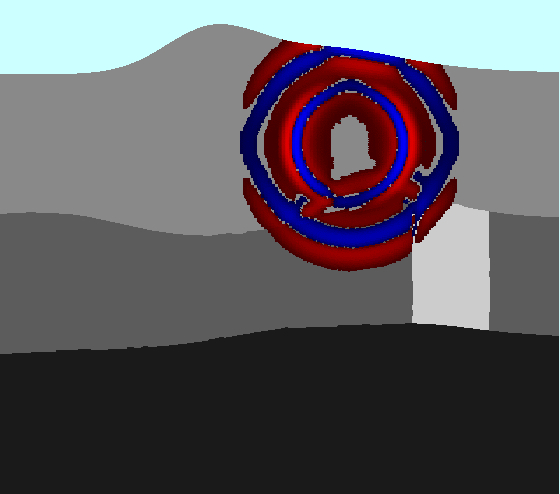
\includegraphics[width=2in]{figures/image0000400.jpg}
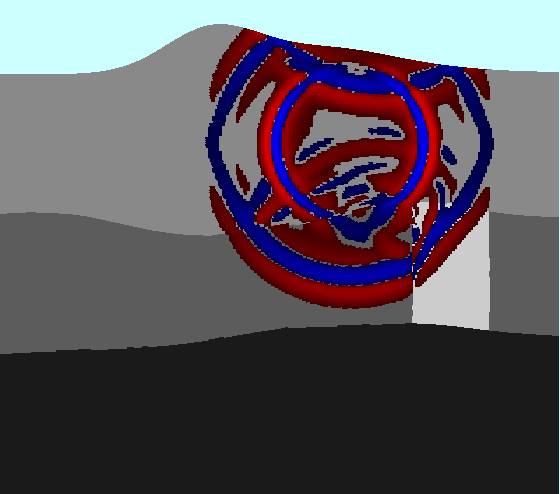
\includegraphics[width=2in]{figures/image0000500.jpg}
\par\end{centering}
\caption{Wavefield snapshots of the default example generated by \texttt{xspecfem2D} when parameter \texttt{output\_color\_image} is set to \texttt{.true.}. To create smaller (subsampled) images you can change double precision parameter \texttt{factor\_subsample\_image = 1.0} to a higher value in file \texttt{DATA/Par\_file}. This can be useful in the case of very large models. The number of pixels of the image in each direction must be smaller than parameter \texttt{NX\_NZ\_IMAGE\_MAX} defined in file \texttt{SETUP/constants.h.in}, again to avoid creating huge images in the case of very large models.}
\label{fig:example.solver}
\end{figure}
%%

\noindent
Please consider these following points, when running the solver:
\begin{itemize}
\item the \texttt{DATA/Par\_file} given with the code works fine, you can use it without any modification to test the code

\item the seismograms \texttt{OUTPUT\_FILES/*.sem*} are simple ASCII files with two columns: time in the first column and amplitude in the second, therefore they can be visualized with any tool you like, for instance "\texttt{gnuplot}"; if you prefer to output binary seismograms in Seismic Unix format (which is a simple binary array dump) you can use parameter SU\_FORMAT, in which case all the seismograms will be written to a single file with the extension *.su.
Depending on your installation of the Seismic Unix package you can use one of these two commands:

surange < Uz\_file\_single.bin 

suoldtonew < Uz\_file\_single.bin | surange

to see the header info. 
Replace \texttt{surange} with \texttt{suxwigb} to see wiggle plots for the seismograms.

\item if you set flag \texttt{assign\_external\_model} to \texttt{.true.} in \texttt{DATA/Par\_file}, the velocity and density model that is given at the end of \texttt{DATA/Par\_file} is then ignored and overwritten by the external velocity and density model that you define yourself in \texttt{define\_external\_model.f90}

\item when compiling with Intel ifort, use "\texttt{-assume byterecl}" option to create binary PNM images displaying the wave field

\item there are a few useful scripts and Fortran routines in directory \texttt{UTILS/}.

\item if you find bugs (or if you have comments or suggestions) please send an email to cig-seismo AT geodynamics.org and the developers will try to fix them and send you an updated version

\item you can find a Fortran code to compute the analytical solution for simple media that we use as a reference in benchmarks in many of our articles at
\urlwithparentheses{http://www.spice-rtn.org/library/software/EX2DDIR}. That code is described in: \cite{BeIfNiSk94}

\end{itemize}

\noindent
The \texttt{SOURCE} file located in the \texttt{DATA/} directory should be edited in the following way:
\begin{description}
\item[source\_surf] Set this flag to \texttt{.true.} to force the source to be located at the surface of the model, otherwise
the source will be placed inside the medium

\item[xs] source location x in meters

\item[zs] source location z in meters

\item[source\_type] Set this value equal to \texttt{1} for elastic forces or acoustic pressure,
set this to \texttt{2} for moment tensor sources.
For a plane wave including converted and reflected waves at the free surface, P wave = 1, S wave = 2, Rayleigh wave = 3;
for a plane wave without converted nor reflected waves at the free surface, i.e. the incident wave only, P wave = 4, S wave = 5.
(incident plane waves are turned on by parameter \texttt{initialfield} in \texttt{DATA/Par\_file}).

\item[time\_function\_type] Choose a source-time function: set this value to \texttt{1} to use a Ricker,
\texttt{2} the first derivative, \texttt{3} a Gaussian, \texttt{4} a Dirac or \texttt{5} a Heaviside source-time function.

\item[f0] Set this to the dominant frequency of the source.
For point-source simulations using a Heaviside source-time function (time\_function\_type "5"),
we recommend setting the source frequency parameter \texttt{f0}
equal to a high value, which corresponds to simulating a step source-time
function, i.e., a moment-rate function that is a delta function.

The \texttt{half duration} of a source is obtained by \texttt{1/f0}.
If the code will use a Gaussian source-time function (time\_function\_type "3")
(i.e., a signal with a shape similar to a `smoothed triangle', as
explained in \citet{KoTr02a} and shown in Fig~\ref{fig:gauss.vs.triangle}), the
source-time function uses a half-width of \texttt{half duration}. We prefer
to run the solver with \texttt{half duration} set to zero and convolve
the resulting synthetic seismograms in post-processing after the run,
because this way it is easy to use a variety of source-time functions.
\citet{KoTr02a} determined
that the noise generated in the simulation by using a step source
time function may be safely filtered out afterward based upon a convolution
with the desired source time function and/or low-pass filtering. Use
the serial code \texttt{convolve\_source\_timefunction.f90} and the
script \texttt{convolve\_source\_timefunction.csh} for this purpose,
or alternatively use signal-processing software packages such as SAC \urlwithparentheses{www.llnl.gov/sac}.
Type
\begin{lyxcode}
make~convolve\_source\_timefunction
\end{lyxcode}
to compile the code and then set the parameter \texttt{hdur} in \texttt{convolve\_source\_timefunction.csh}
to the desired half-duration.
%%
\begin{figure}[htbp]
\noindent \begin{centering}
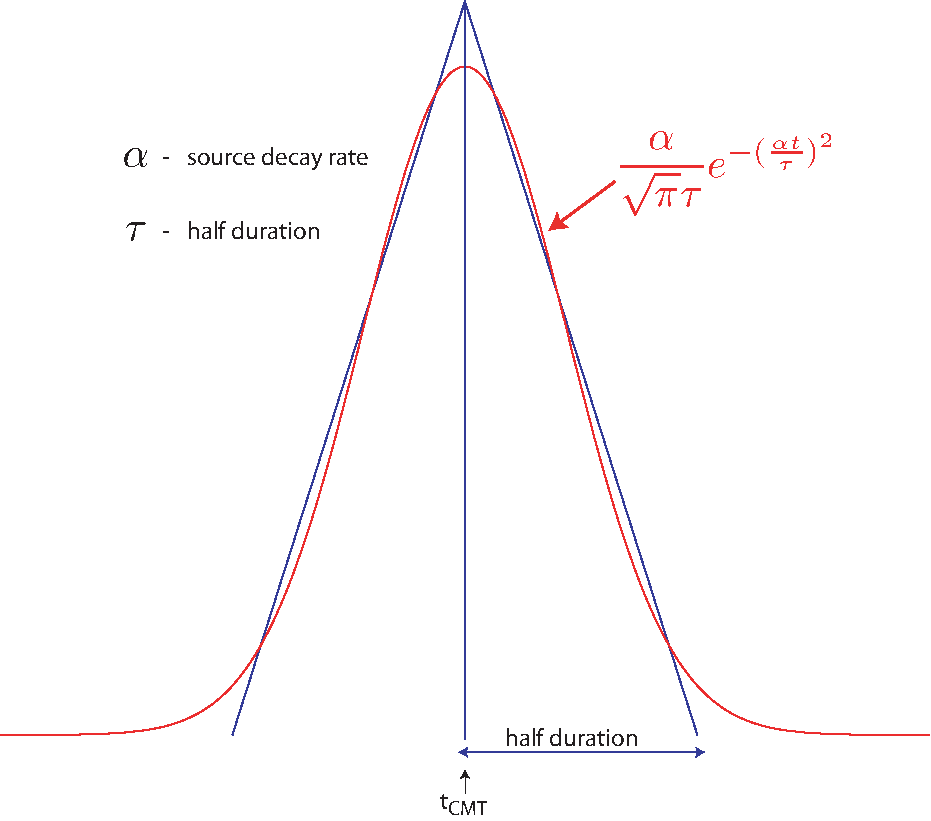
\includegraphics[width=3in]{figures/gauss_vs_triangle_mod.pdf}
\par\end{centering}
\caption{Comparison of the shape of a triangle and the Gaussian function actually
used.}
\label{fig:gauss.vs.triangle}
\end{figure}
%%

\item[t0] For single sources, we recommend to set the time shift parameter \texttt{t0} equal to $0.0$.
The time shift parameter would simply apply
an overall time shift to the synthetics (according to the time shift of the first source), something that can be done
in the post-processing. This time shift parameter can be non-zero when using multiple sources.

\item[anglesource] angle of the source (for a force only); for a plane wave, this is the incidence angle. For moment tensor sources this parameter is unused.

\item[Mxx,Mzz,Mxz] Moment tensor components (valid only for moment tensor sources, source\_type "2").
Note that the units for the components of a moment tensor source are different in SPECFEM2D and in SPECFEM3D:
\begin{description}
\item[SPECFEM3D:] in SPECFEM3D the moment tensor components are in dyne*cm
\item[SPECFEM2D:] in SPECFEM2D the moment tensor components are in N*m
\end{description}

\item[factor] amplification factor

\end{description}
Note, the zero time of the simulation corresponds to the center of the triangle/Gaussian,
or the centroid time of the earthquake. The start time of the simulation
is $t=-1.2*\texttt{half duration} + \texttt{t0}$ (the factor 1.2 is to make sure the moment
rate function is very close to zero when starting the simulation; Heaviside functions use a factor 2.0),
the half duration is obtained by 1/f0.
If you prefer, you can fix this start time by setting the parameter \texttt{USER\_T0} in the \texttt{constants.h} file
to a positive, non-zero value. The simulation in that case would start at a starting time equal to \texttt{-USER\_T0}.




%------------------------------------------------------------------------------------------------%
\subsection*{Caution}
%------------------------------------------------------------------------------------------------%

See file \texttt{todo\_list\_please\_dont\_remove.txt} for a list of known bugs, problems, or missing options.

%------------------------------------------------------------------------------------------------%

\subsection*{Coupled Simulations}

%------------------------------------------------------------------------------------------------%

The code supports acoustic/elastic, acoustic/poroelastic, elastic/poroelastic,
and acoustic,elastic/poroelastic simulations.\\

\noindent
Elastic/poroelastic coupling supports anisotropy, but not attenuation for the
elastic material.


%------------------------------------------------------------------------------------------------%
\section{How to run P-SV or SH (membrane) wave simulations}
%------------------------------------------------------------------------------------------------%

For elastic materials, you have these additional options:
\begin{description}
\item[P-SV:]
To run a P-SV waves calculation propagating in the x-z plane,
set \texttt{p\_sv = .true.} in the \texttt{Par\_file}.

\item[SH:]
To run a SH (membrane) waves calculation traveling in the x-z plane with a
y-component of motion, set \texttt{p\_sv = .false.}

\end{description}
This feature is only implemented for elastic materials and sensitivity kernels
can be calculated (see \cite{TaLiTr07} for details on membrane
surface waves).


A useful Python script called \texttt{SEM\_save\_dir.py}, written by Paul Cristini from
Laboratoire de Mecanique et d'Acoustique, CNRS, Marseille, France, is provided.
It allows one to automatically save all the parameters and results of a given simulation.

%------------------------------------------------------------------------------------------------%
\section{How to use anisotropy}
%------------------------------------------------------------------------------------------------%

\begin{flushleft}
Following \cite{CaKoKo88}, we use the classical reduced Voigt notation \citep{Hel94,Car07}:
\end{flushleft}
%%%
\noindent \begin{centering}
{\small 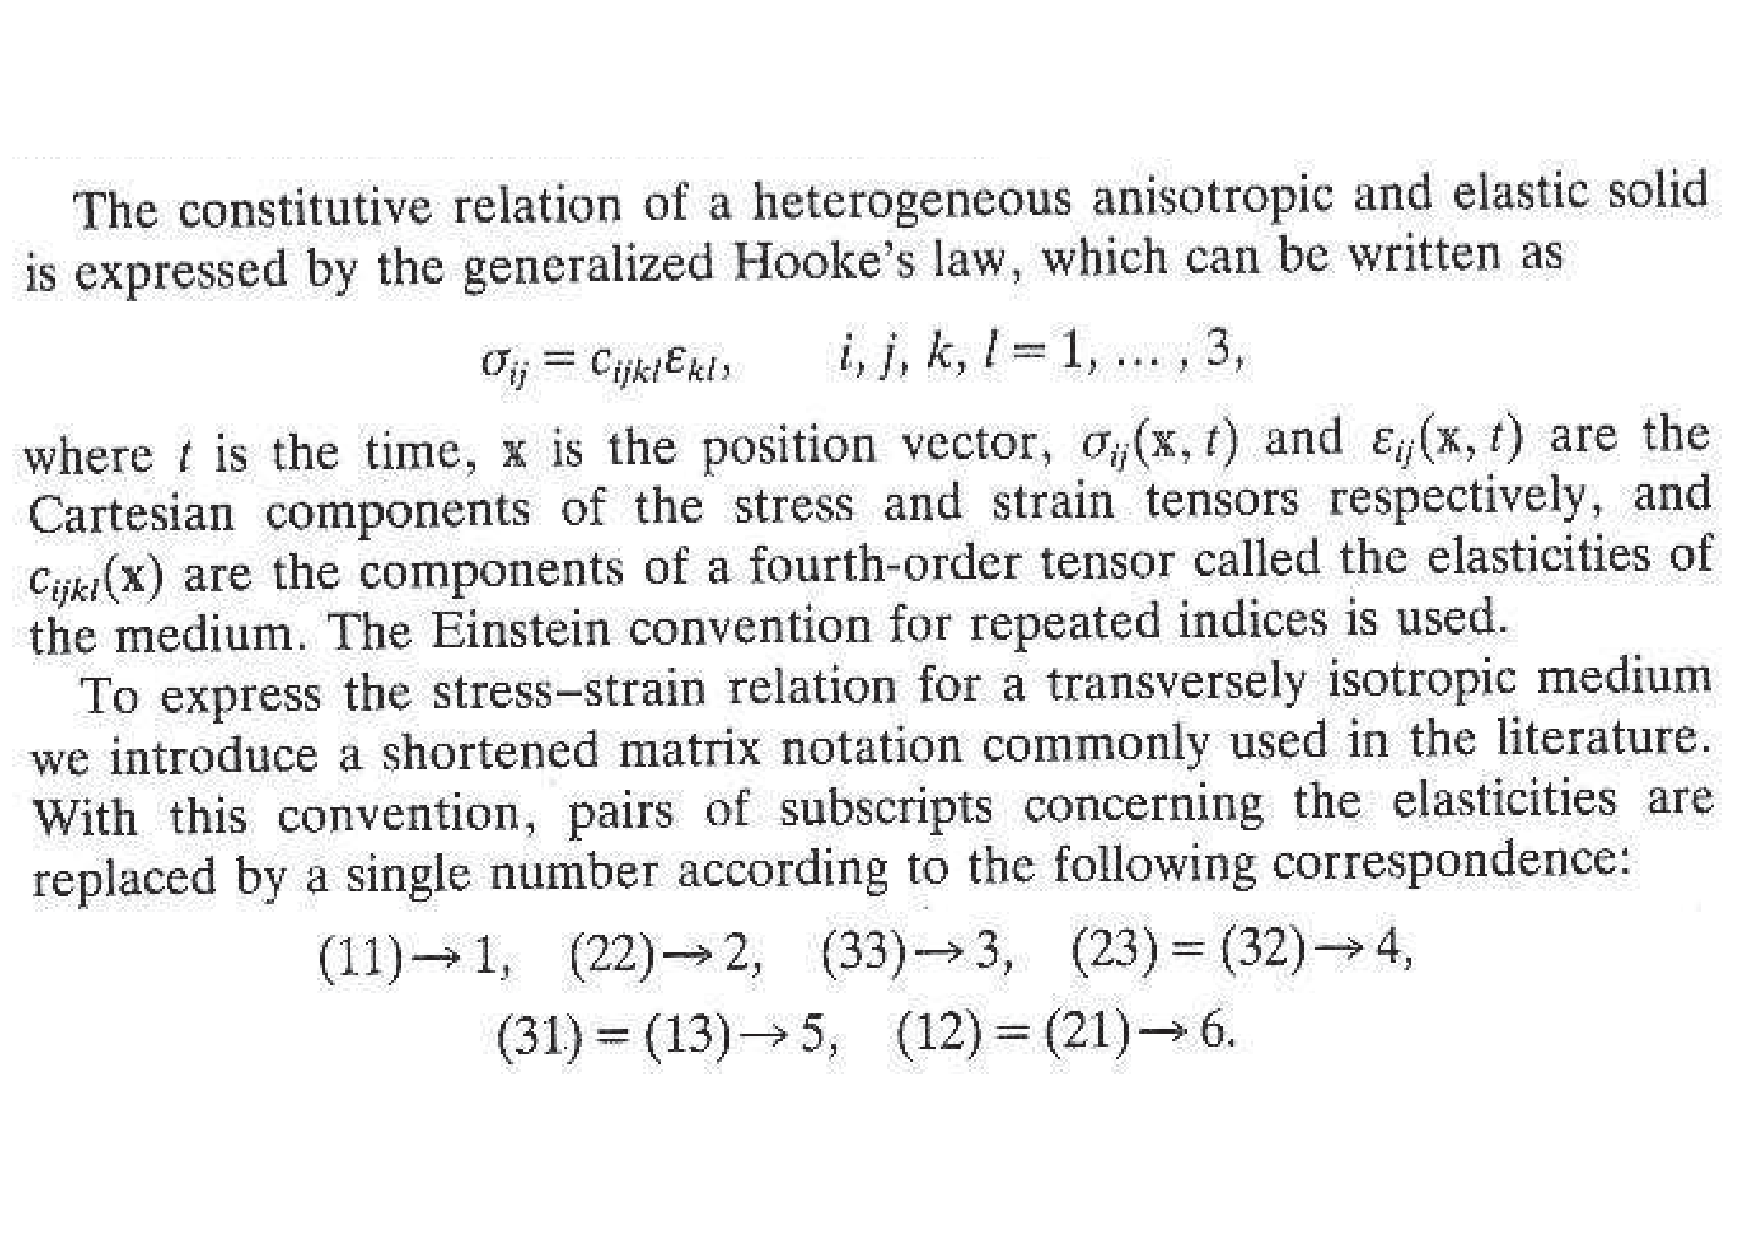
\includegraphics[width=4.2in,trim=0 2.6cm 0 2.6cm]{figures/Carcione_et_al_aniso_1988_image.pdf} }
\par\end{centering}{\small \par}
%%%

\noindent
Thus in the most general 2D case we have the following convention for the stress-strain relationship:
%
\begin{verbatim}
! implement anisotropy in 2D
sigma_xx = c11*dux_dx + c15*(duz_dx + dux_dz) + c13*duz_dz
sigma_zz = c13*dux_dx + c35*(duz_dx + dux_dz) + c33*duz_dz
sigma_xz = c15*dux_dx + c55*(duz_dx + dux_dz) + c35*duz_dz
\end{verbatim}
%
where the notations are for instance \texttt{duz\_dx = d(Uz) / dx}.


%------------------------------------------------------------------------------------------------%
\section{How to use poroelasticity}
%------------------------------------------------------------------------------------------------%

Check the following new inputs in \texttt{Par\_file}:
\begin{description}
\item In section {\bf "\# geometry of model and mesh description"}:\\
\texttt{TURN\_VISCATTENUATION\_ON}, \texttt{Q0}, and \texttt{FREQ0} deal with viscous damping in a poroelastic medium.
\texttt{Q0} is the quality factor set at the central frequency \texttt{FREQ0}. For more details
see \cite{MoTr08}.

\item In section {\bf "\# time step parameters"}:\\
\texttt{SIMULATION\_TYPE} defines the type of simulations \\
(1) forward simulation \\
(2) UNUSED (purposely, for compatibility with the numbering convention used in our 3D codes) \\
(3) adjoint method and kernels calculation

\item In section {\bf "\# source parameters"}:\\
The code now support multi sources.
\texttt{NSOURCE} is the number of source.
Parameters of the sources are displayed in the file \texttt{SOURCE}, which must be
in the directory \texttt{DATA/}. The components of a moment tensor source must be given in N.m,
not in dyne.cm as in the \texttt{DATA/CMTSOLUTION} source file of the 3D version of the code.
%%%
{\small }%
\begin{figure}[htbp]
\noindent \begin{centering}
{\small 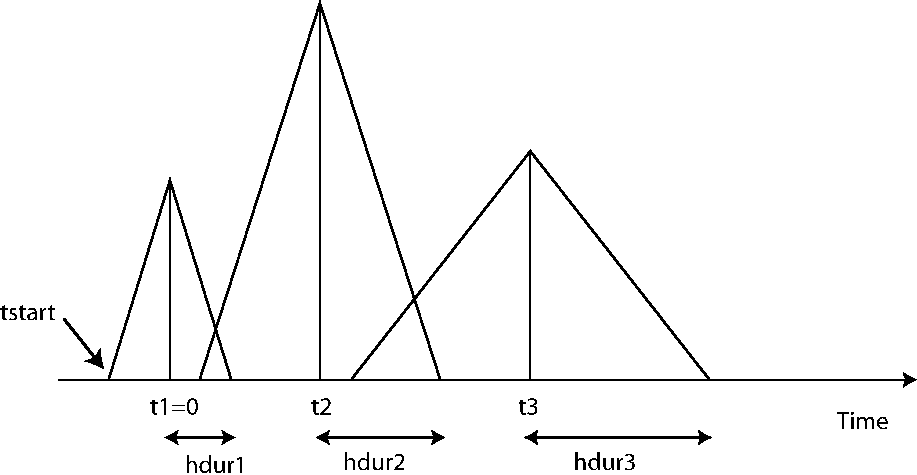
\includegraphics[width=5in]{figures/source_timing.pdf} }
\par\end{centering}{\small \par}
\caption{Example of timing for three sources. The center of the first source
triangle is defined to be time zero. Note that this is NOT in general
the hypocentral time, or the start time of the source (marked as tstart).
The time shift parameter \texttt{t0} in the \texttt{SOURCE} file
would be t1(=0), t2, t3 in this case, and the half-duration parameter, resp. \texttt{f0},
would be hdur1=1/f0\_1, hdur2=1/f0\_2, hdur3=1/f0\_3 for the sources 1, 2, 3 respectively.}
{\small \label{fig:source_timing} }
\end{figure}
{\small \par}
%%%


\item In section {\bf "\# receiver line parameters for seismograms"}:\\
\texttt{SAVE\_FORWARD} determines if the last frame of a forward simulation is saved (\texttt{.true.}) or not (\texttt{.false})

\item In section {\bf "\# define models...."}:\\
There are three possible types of models:\\
 \texttt{I}:   (model\_number 1 rho Vp Vs 0 0 QKappa Qmu 0 0 0 0 0 0) or\\
 \texttt{II}:  (model\_number 2 rho c11 c13 c15 c33 c35 c55 0 0 0 0 0 0) or\\
 \texttt{III}: (model\_number 3 rhos rhof phi c kxx kxz kzz Ks Kf Kfr etaf mufr Qmu). \\

For istropic elastic/acoustic material use \texttt{I} and set Vs to zero to make a given model acoustic, for anisotropic elastic use \texttt{II},
and for isotropic poroelastic material use \texttt{III}. The mesh can contain acoustic, elastic, and poroelastic models simultaneously.
rho\_s = solid density\\
rho\_f = fluid density\\
phi = porosity\\
tort = tortuosity\\
permxx = xx component of permeability tensor\\
permxz = xz,zx components of permeability tensor\\
permzz = zz component of permeability tensor\\
kappa\_s = solid bulk modulus\\
kappa\_f= fluid bulk modulus\\
kappa\_fr= frame bulk modulus\\
eta\_f = fluid viscosity\\
mu\_fr = frame shear modulus\\
Qmu = shear quality factor\\

Note: for the poroelastic case, mu\_s is irrelevant.
For details on the poroelastic theory see \cite{MoTr08}.

\end{description}

\texttt{get\_poroelastic\_velocities.f90} allows to compute cpI, cpII, and cs function of
the source dominant frequency. Notice that for this calculation we use permxx
and the dominant frequency of the first source , f0(1). Caution if you use
several sources with different frequencies and if you consider anistropic
permeability.

%------------------------------------------------------------------------------------------------%
\section{How to set plane waves as initial conditions}
To simulate propagation of incoming plane waves in the simulation domain, initial conditions based on analytical formulae of plane waves in homogenous model need to be set. No additional body or boundary forces are required. To set up this senario:
\begin{description}
\item{\verb+Par_file+:}
  \begin{itemize}
  \item switch on \verb+initialfield = .true. +
  \item at this point setting \verb+add_bielak_condition+ does not seem to help with absorbing boundaries, therefore, it should be turned off.
  \end{itemize}
\item{\verb+SOURCE+:}
  \begin{itemize}
  \item \verb+zs+ has to be the same as the height of the simulation domain defined in \verb+interfacesfile+.
  \item \verb+xs+ is the x-coordinate of the intersection of the initial plane wave front with the free surface.
  \item \verb+source_type+ = 1 for a plane P wave, 2 for a plane SV wave, 3 for a Rayleigh wave.
  \item \verb+angleforce+ can be negative to indicate a plane wave incident from the right (instead of the left)
  \end{itemize}
\end{description}

%------------------------------------------------------------------------------------------------%
\section{How to choose the time step}

Three different explicit conditionally-stable time schemes can be used for elastic, acoustic (fluid) or coupled elastic/acoustic media:
the Newmark method, the low-dissipation and low-dispersion fourth-order six-stage Runge-Kutta method (LDDRK4-6) presented in \cite{BeBoBa06},
and the classical fourth-order four-stage Runge-Kutta (RK4) method.
Currently the last two methods are not implemented for poro-elastic media.
According to \cite{DeSe10} and \cite{BeBoBa06}, with different degrees $N=NGLLX-1$ of the GLL basis funtions the CFL bounds are given in the following tables.
Note that by default the SPECFEM solver uses $NGLLX = 5$ and thus a degree $N = 4$, which is thus the value you should use
in most cases in the following tables.
You can directly compare these values with the value given in sentence 'Max stability for P wave velocity' in file
\texttt{output\_solver.txt} to see whether you set the correct $\Delta_t$ in \texttt{Par\_file} or not.
For elastic simulation, the
CFL value given in \texttt{output\_solver.txt} does not consider the Vp/Vs ratio, but the CFL limit slight decreases when Vp/Vs increases.
In viscoelastic simulations the CFL limit does not change compared to the elastic case because we use a rational approximation of a constant quality factor Q, which has no attenuation effect on zero-frequency waves.
Additionally, if you use C-PML absorbing layers in your simulations, which are implemented for the Newmark and LDDRK4-6 techniques but not for the classical RK4), the CFL upper limit decreases to approximately $95\%$ of the limit without absorbing layers in the case of Newmark and to $85\%$ in the case of LDDRK4-6.
\begin{table}[hb]
\caption{CFL upper bound for an acoustic (fluid) simulation.}
% title of Table
\centering
% used for centering table
\begin{tabular}{c c c c}
% centered columns (4 columns)
\hline\hline
%inserts double horizontal lines
Degree $N$ & Newmark & LDDRK4-6 & RK4 \\ [0.5ex]
% inserts table
%heading
\hline
% inserts single horizontal line
1 & 0.709 & 1.349 & 1.003 \\
2 & 0.577 & 1.098 & 0.816 \\
3 & 0.593 & 1.129 & 0.839 \\
\red{4} & \red{0.604} & \red{1.150} & \red{0.854} \\
5 & 0.608 & 1.157 & 0.860 \\
6 & 0.608 & 1.157 & 0.860 \\
7 & 0.608 & 1.157 & 0.860 \\
8 & 0.607 & 1.155 & 0.858 \\
9 & 0.607 & 1.155 & 0.858 \\
10 & 0.607 & 1.155 & 0.858 \\ [1ex]
% [1ex] adds vertical space
\hline
%inserts single line
\end{tabular}
\label{table:CFLacoustic}
% is used to refer this table in the text
\end{table}
%
\clearpage
\noindent
\begin{table}[t]
\caption{CFL upper bound for an elastic simulation with Vp/Vs = $\sqrt{2}$.}
% title of Table
\centering
% used for centering table
\begin{tabular}{c c c c}
% centered columns (4 columns)
\hline\hline
%inserts double horizontal lines
Degree $N$ & Newmark & LDDRK4-6 & RK4 \\ [0.5ex]
% inserts table
%heading
\hline
% inserts single horizontal line
1 & 0.816 & 1.553 & 1.154 \\
2 & 0.666 & 1.268 & 0.942 \\
3 & 0.684 & 1.302 & 0.967 \\
\red{4} & \red{0.697} & \red{1.327} & \red{0.986} \\
5 & 0.700 & 1.332 & 0.990 \\
6 & 0.700 & 1.332 & 0.990 \\
7 & 0.700 & 1.332 & 0.990 \\
8 & 0.699 & 1.330 & 0.989 \\
9 & 0.698 & 1.328 & 0.987 \\
10 & 0.698 & 1.328 & 0.987 \\ [1ex]
% [1ex] adds vertical space
\hline
%inserts single line
\end{tabular}
\label{table:CFLelastic}
% is used to refer this table in the text
\end{table}

%------------------------------------------------------------------------------------------------%

%------------------------------------------------------------------------------------------------%

\chapter{Adjoint Simulations}

%------------------------------------------------------------------------------------------------%


%------------------------------------------------------------------------------------------------%
\section{How to obtain Finite Sensitivity Kernels}
%------------------------------------------------------------------------------------------------%

\begin{enumerate}
\item[1.] Run a forward simulation: \\
=> \texttt{SIMULATION\_TYPE = 1} \\
=> \texttt{SAVE\_FORWARD = .true.}\\
=> \texttt{seismotype = 1} (we need to save the displacement fields to later on derive the
adjoint source. Note: if the user forgets it, the program corrects it when reading the proper
\texttt{SIMULATION\_TYPE} and \texttt{SAVE\_FORWARD} combination and a warning message appears in the ouput
file)\\

Important output files (for example, for the elastic case, P-SV waves): \\s
\texttt{absorb\_elastic\_bottom*****.bin}\\
\texttt{absorb\_elastic\_left*****.bin}\\
\texttt{absorb\_elastic\_right*****.bin}\\
\texttt{absorb\_elastic\_top*****.bin}\\
\texttt{lastframe\_elastic*****.bin}\\
\texttt{S****.AA.BXX.semd}\\
\texttt{S****.AA.BXZ.semd}\\

\item[2.] Define the adjoint source: \\
Use \texttt{adj\_seismogram.f90}\\
Edit to update \texttt{NSTEP}, \texttt{nrec}, \texttt{t0}, \texttt{deltat}, and the position of the cut to pic
any given phase if needed (\texttt{tstart},\texttt{tend}), add the right number of stations, and
put one component of the source to zero if needed.
The ouput files of \texttt{adj\_seismogram.f90} are \texttt{S****.AA.BXX.adj} and \texttt{S****.AA.BXZ.adj}, for P-SV waves (and
\texttt{S****.AA.BXY.adj}, for SH (membrane) waves). Note that you will need these three
files (\texttt{S****.AA.BXX.adj}, \texttt{S****.AA.BXY.adj} and \texttt{S****.AA.BXZ.adj}) to be present in the \texttt{SEM/} directory
together with the \texttt{absorb\_elastic\_****.bin} and \texttt{lastframe\_elastic.bin} files to be read
when running the adjoint simulation.\\

\item[3.] Run the adjoint simulation: \\
Make sure that the adjoint source files absorbing boundaries and last frame files are
in the \texttt{OUTPUT\_FILES/} directory.\\
=> \texttt{SIMULATION\_TYPE = 3}\\
=> \texttt{SAVE\_FORWARD = .false.}\\

Output files (for example for the elastic case):\\
\texttt{snapshot\_rho\_kappa\_mu*****}\\
\texttt{snapshot\_rhop\_alpha\_beta*****}\\
which are the primary moduli kernels and the phase velocities kernels respectively, in ascii format
and at the local level, that is as "kernels(i,j,ispec)".

\end{enumerate}

\subsection*{Remarks about adjoint runs and solving inverse problems}

% This from Carl Tape:
SPECFEM2D can produce the gradient of the misfit function for a
tomographic inversion, but options for using the gradient within an
iterative inversion are left to the user (e.g., conjugate-gradient,
steepest descent). The plan is to include some examples in the future.\\

% This from Yang Luo:
The algorithm is simple:

\begin{enumerate}
\item[1.] calculate the forward wave field $\mathbf{s}(x,t)$
\item[2.] calculate the adjoint wave field $\mathbf{s}^\dagger(x,t)$
\item[3.] calculate their interaction $\mathbf{s}(x,t) \cdot \mathbf{s}^\dagger(x,T-t)$ (these symbolic, temporal and spatial derivatives should be included)
\item[4.] integrate the interactions, which is summation in the code.
\end{enumerate}

That is all. Step 3 has some tricks in implementation, but which can be skipped by regular users.\\

If you look into SPECFEM2D, besides "rhop\_ac\_kl" and "rho\_ac\_kl",
there are more variables such as "kappa\_ac\_kl" and "rho\_el\_kl" etc.
"rho" denotes density $\rho$ ("kappa" for bulk modulus $\kappa$ etc.),
"ac" denotes acoustic ("el" for elastic),
"kl" means kernel (and you may find "k" as well, which is the interaction at each time step, i.e., before doing time integration).

\subsection*{Caution}

Please note that
\begin{itemize}
\item at the moment, adjoint simulations do not support anisotropy, attenuation, and viscous damping.

\item you will need \texttt{S****.AA.BXX.adj}, \texttt{S****.AA.BXY.adj} and \texttt{S****.AA.BXZ.adj}
to be present in directory \texttt{SEM/} even if you are just running an acoustic or
poroelastic adjoint simulation.\\
\texttt{S****.AA.BXX.adj} is the only relevant component for an acoustic case.\\
\texttt{S****.AA.BXX.adj} and \texttt{S****.AA.BXZ.adj} are the only relevant components for a
poroelastic case.
\end{itemize}


%------------------------------------------------------------------------------------------------%

\chapter{Oil and gas industry simulations}

%------------------------------------------------------------------------------------------------%

The SPECFEM2D package provides compatibilities in industrial (oil and gas industry) types of simulations.
These features include importing Seismic Unix (SU) format wavespeed models into SPECFEM2D,
outputing seismograms also in SU format with a few key parameters defined in the trace headers
and reading adjoint sources in SU format etc.
There is one example given in EXAMPLES/INDUSTRIAL\_FORMAT, which you can follow.

We also changed the relationship between adjoint potential and adjoint displacement in fluid region
(the relationship between forward potential and forward displacement remains the same as previsouly defined).
The new definition is critical when there are adjoint sources (in other words, receivers) in the acoustic domain,
and is the direct consequence of the optimization problem.
\begin{eqnarray*}
\mathbf{s}&\equiv&\frac{1}{\rho}~\mathbf{\nabla}\phi \\
p&\equiv&-\kappa(\nabla\cdot\mathbf{s}) =-\partial_t^2\phi \\
\quad\\
\partial_t^2\mathbf{s}^\dagger&\equiv&-\frac{1}{\rho}~\mathbf{\nabla}\phi^\dagger\\
p^\dagger&\equiv&-\kappa(\nabla\cdot\mathbf{s}^\dagger)=\phi^\dagger
\end{eqnarray*}



%------------------------------------------------------------------------------------------------%

\chapter*{Acknowledgments}

%------------------------------------------------------------------------------------------------%

The Gauss-Lobatto-Legendre subroutines in \texttt{gll\_library.f90}
are based in part on software libraries from the Massachusetts Institute
of Technology, Department of Mechanical Engineering (Cambridge, Massachusetts, USA).
The non-structured global numbering software was provided by Paul
F. Fischer (Brown University, Providence, Rhode Island, USA, now at Argonne National Laboratory, USA).


Please e-mail your feedback, questions, comments, and suggestions
to Jeroen Tromp \urlwithparentheses{jtromp-AT-princeton.edu} or to the CIG Computational Seismology Mailing List \urlwithparentheses{cig-seismo@geodynamics.org}.


%------------------------------------------------------------------------------------------------%

\chapter*{Copyright}

%------------------------------------------------------------------------------------------------%

Main historical authors: Dimitri Komatitsch and Jeroen Tromp

Princeton University, USA,
and CNRS / INRIA / University of Pau, France

$\copyright$ Princeton University and CNRS / INRIA / University of Pau, July 2012


%------------------------------------------------------------------------------------------------%

\bibliography{bibliography}

%------------------------------------------------------------------------------------------------%
%------------------------------------------------------------------------------------------------%


\appendix


%------------------------------------------------------------------------------------------------%

\chapter{\label{cha:Troubleshooting}Troubleshooting}

%------------------------------------------------------------------------------------------------%


\section*{FAQ}

\begin{description}
\item[Regarding the structure of some of the database files] : \newline

{\bf Question:} Can anyone tell me what the columns of the SPECFEM2D boundary
condition files in \texttt{SPECFEM2D/DATA/}~\\
\texttt{Mesh\_canyon} are?\\

\texttt{SPECFEM2D/DATA/Mesh\_canyon/canyon\_absorbing\_surface\_file} \\
\texttt{SPECFEM2D/DATA/Mesh\_canyon/canyon\_free\_surface\_file}

{\bf Answer:} \texttt{canyon\_absorbing\_surface\_file} refers to parameters related to the
absorbing conditions:
The first number (180) is the number of absorbing elements (nelemabs in the
code).
Then the columns are:\\
column 1 = the element number\\
column 2 = the number of nodes of this element that form the absorbing surface\\
column 3 =  the first node\\
column 4 = the second node\\

\texttt{canyon\_free\_surface\_file} refers to the elements of the free surface
(relevant for enforcing free surface condition for acoustic media):
The first number (160) is the number of  elements of the free surface.
Then the columns are (similar to the absorbing case):\\
column 1 = the element number\\
column 2 = the number of nodes of this element that form the absorbing surface\\
column 3 =  the first node\\
column 4 = the second node\\

Concerning the free surface description file, nodes/edges pertaining to
elastic elements are discarded when the file is read (if for whatever
reason it was simpler to include all the nodes/edges on one side of a
studied area and that there are among them some elements that are
elastic elements, only the nodes/edges of acoustic elements are kept).

These files are opened and read in \texttt{meshfem2D.F90} using subroutines
\texttt{read\_abs\_surface()} and \texttt{read\_}~\\
\texttt{acoustic\_surface()}, which are in \texttt{part\_unstruct.F90}





\end{description}


%------------------------------------------------------------------------------------------------%

\end{document}

